\section{Test cases}

\subsection{Game-Explorer}

\begin{tabular}{cll}

\hline
\textbf{Test} & \textbf{Description} & \textbf{Tested Functionalities} \\
\hline
/T010/ & Select a game & \ref{FR:GE010}, \ref{FR:GE040} \\
/T020/ & Start a game & \ref{FR:GE020} \\
/T030/ & Use the help function & \ref{FR:GE030} \\
/T040/ & Add new game & \ref{FR:GE010}, \ref{FR:GE050} \\
\hline

\end{tabular}

\subsection{Games}

\subsubsection{\graphcoloring}

\begin{tabular}{cll}

\hline
\textbf{Test} & \textbf{Description} & \textbf{Tested Functionalities} \\
\hline
/T110/ & Start the game & \ref{FR:F010}, \ref{FR:F060},\\
 & & \ref{FR:GU010} \\
/T120/ & Save/load a game & \ref{FR:G010}, \ref{FR:G020}\\
/T130/ & Color an uncolored vertex & \ref{FR:F020}, \ref{FR:F040}, \\
 & & \ref{FR:GU020}, \ref{FR:GU040}\\
/T140/ & Color a colored vertex & \\
/T150/ & Color a vertex next to a colored one in the same color & \\
/T160/ & Win/Lose a game & \\
\hline

\end{tabular}

\subsubsection{\twixt}

\begin{tabular}{cll}

\hline
\textbf{Test} & \textbf{Description} & \textbf{Tested Functionalities} \\
\hline
/T210/ & Start the game & \ref{FR:F010}, \ref{FR:F060}, \ref{FR:GU010} \\
/T220/ & Save/load a game & \ref{FR:G010}, \ref{FR:G020} \\
/T230/ & Place edges/vertices & \ref{FR:F020}, \ref{FR:F030}, \ref{FR:GU020}, \\ 
& & \ref{FR:GU040} \\
/T240/ & Place an edge across an opponent's one & \ref{FR:F070} \\
/T250/ & Place a vertex on an already occupied field & \\
/T260/ & Win/Lose a game & \ref{FR:F050} \\
\hline

\end{tabular}

\subsection{Test scenarios}

\subsubsection{Add a game to the Game-Explorer}

Alice starts the Game-Explorer and adds a new game by using the 'Add'-function. Then Alice selects the game in the list in order to look at the screenshot and the desription of the game. Still not convinced, Alice uses the help function to gain an insight in how the game works. Then Alice starts the game.

\subsubsection{Play {\graphcoloring} Single-Player} \label{T:GCSingle}

Bob starts {\graphcoloring} with the Game-Explorer. Bob selects the color red and colors vertex 1. Then Bob selects blue, colors vertex 3 and 4 and tries to color vertex 2, but it stays uncolored. A status bar displays an error message for a few seconds. Bob then selects green and colors vertex 2. A win message is displayed and the next level is loaded.

\subsubsection{Play {\graphcoloring} Multiplayer} \label{T:GCMulti}

Carol and Dave start {\graphcoloring} with the Game-Explorer. Carol selects the color blue and colors vertex 2. Dave selects red and colors vertex 4. Carol selects green and tries to color vertex 2, but it stays blue. Carol then colors vertex 3. Since no valid move is possible anymore, a win message for Carol is displayed and another graph is loaded.

\begin{figure}[h!]
	\centering
	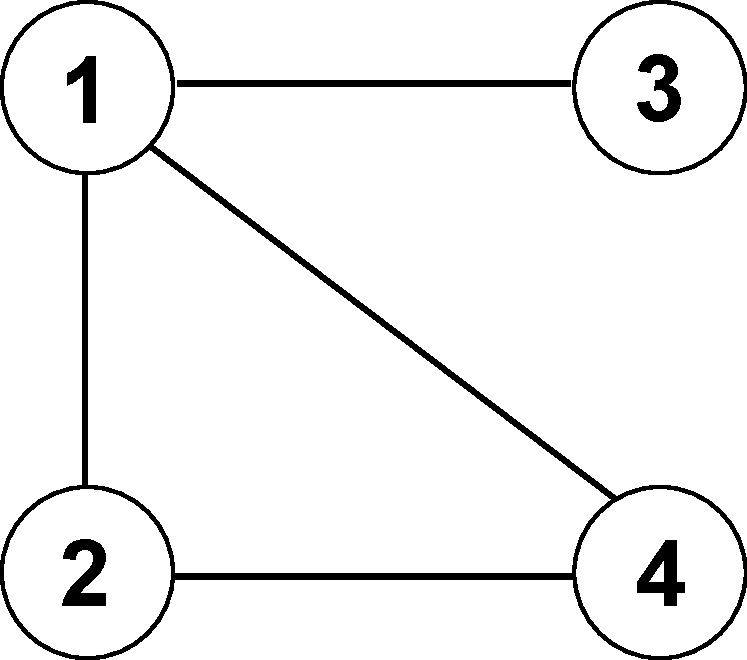
\includegraphics[width=0.25\textwidth]{testgraph.pdf}
	\caption{Graph the scenarios \ref{T:GCSingle} and \ref{T:GCMulti} are based on}
	\label{img:ACTDEV}
\end{figure}

\subsubsection{Play \twixt}

Carol and Dave start {\twixt} with the Game-Explorer. They take turns placing vertices or edges until one of them has build a path from one to the other side. Then they close the game.
